\section{Formalisme théorique et interactions}\label{chapter-MS-MSSM-section-formalisme}
Il ne suffit pas de lister les particules fondamentales pour obtenir un modèle, il faut également décrire leur dynamique, \ie\ la façon dont ces particules interagissent. 
Pour cela, le modèle standard se base sur la théorie quantique des champs. Une particule n'est pas un \og objet ponctuel \fg{} comme en mécanique classique, mais une excitation d'un champ quantique relativiste. Il s'agit alors de décrire l'évolution de ces excitations.
\par
%Les lois de la mécanique classique ne sauraient remplir ce rôle.
Le comportement des particules fondamentales est obtenu par l'application des équations d'Euler-Lagrange au lagrangien du modèle standard.
Afin de comprendre pourquoi ce formalisme mathématique permet effectivement d'obtenir l'évolution des champs quantiques relativistes décrivant les particules, la section suivante consiste en une brève introduction du lagrangien dans le cas de la mécanique classique, suivie d'une généralisation au cas du modèle standard.
\subsection{Introduction au formalisme du lagrangien}\label{chapter-MS-MSSM-section-formalisme-subsec-into_lagrangien}
\subsubsection{Lagrangien et principe de moindre action}%\label{chapter-MS-MSSM-section-formalisme-subsec-into_lagrangien-subsubsec-lagrangien_meca_classique}
Soit une particule de masse $m$, soumise à une force $F$ prise ici constante à des fins d'illustration, se déplaçant dans le temps le long d'une dimension $x$, d'un point $A$ à $t=0$ à un point $B$ à $t=\tau$, comme illustré sur la figure~\ref{fig-ptc_classique_ptA_to_pt_B}.
\par 
La trajectoire de cette particule peut être déterminée à l'aide du principe fondamental de la dynamique, ou seconde loi de Newton, qui s'exprime simplement dans ce cas sous la forme
\begin{equation}
m\dv[2]{x}{t} = F
\mend
\end{equation}
La position de la particule à tout instant est alors obtenue par double intégration selon le temps,
\begin{equation}
x (t) = x_0 + v_0 t + \frac{1}{2}\frac{F}{m}t^2
\end{equation}
avec
$x_0$ et $v_0$ les position et vitesse de la particule à l'instant $t=0$.
\begin{figure}[h]
\centering

\subcaptionbox{Particule classique.\label{fig-ptc_classique_ptA_to_pt_B}}[.45\textwidth]
{\begin{tikzpicture}
\draw [thick, domain=0:4,samples=100,smooth] plot(\x, {16/5-\x*\x/5}) coordinate (B) ;
\draw (0, 16/5) coordinate (A);
\fill (A) circle (1pt);
\fill (B) circle (1pt);
\draw (A) node [left] {$A$};
\draw (B) node [right] {$B$};
\draw [->] (-.7,-.2)--+(5.5,0) node [right] {$t$};
\draw [->] (-.7,-.2)--+(0,3.5) node [above] {$x$};

\draw (0,-.1)--+(0,-.2) node [below] {$0$};
\draw (4,-.1)--+(0,-.2) node [below] {$\tau$};
\end{tikzpicture}}
\hfill
\subcaptionbox{Particule quantique.\label{fig-ptc_quantique_ptA_to_pt_B}}[.45\textwidth]
{\begin{tikzpicture}
\draw [domain=0:4,samples=100,smooth] plot(\x, {16/5-\x*\x/5}) coordinate (B) ;
\draw [dashed, domain=0:4,samples=10,smooth] plot(\x, {16/5-\x*\x/5+(rand)*\x*(4-\x)/5});
\draw (0, 16/5) coordinate (A);
\draw [dotted] (A) to [out=0, in = 90] (2,1.5) arc (360:90:.5) to [out=0, in = 90] (B);
\fill (A) circle (1pt);
\fill (B) circle (1pt);
\draw (A) node [left] {$A$};
\draw (B) node [right] {$B$};
\draw [->] (-.7,-.2)--+(5.5,0) node [right] {$t$};
\draw [->] (-.7,-.2)--+(0,3.5) node [above] {$x$};

\draw (0,-.1)--+(0,-.2) node [below] {$0$};
\draw (4,-.1)--+(0,-.2) node [below] {$\tau$};
\end{tikzpicture}}

\caption[Trajectoires d'une particule.]{Trajectoires d'une particule se déplaçant au cours du temps d'un point $A$ à un point $B$.}
\label{fig-ptc_ptA_to_pt_B}
\end{figure}
\par
Or, cette méthode ne permet pas de décrire le comportement des particules fondamentales.
En effet, à leur échelle, la mécanique quantique prévaut et il n'est pas possible, lorsque l'on observe une particule à un point $A$ puis à un point $B$, de déterminer la trajectoire exacte suivie par cette particule.
En effet,
une particule quantique détectée
en $A$ à $t=0$ puis en $B$ à $t=\tau$
a suivi \emph{toutes les trajectoires} reliant ces deux points
aussi farfelues soient-elles,
y compris celles revenant en arrière dans le temps,
comme illustré en figure~\ref{fig-ptc_quantique_ptA_to_pt_B}.
Utiliser une loi pouvant donner $x(t)$ n'est donc pas pertinent en mécanique quantique.
\par
Il existe toutefois un autre principe physique toujours en place en mécanique quantique, la conservation de l'énergie.
Dans le cas de la particule précédemment décrit, il s'agit de la somme de son énergie cinétique $T$ et de son énergie potentielle $V$, \ie
\begin{equation}
E = T + V = \cste
\end{equation}
où $T$ dépend uniquement de la vitesse de la particule et $V$ uniquement de sa position. %Cette quantité est conservée au cours du temps.
Il en va ainsi de même pour les moyennes temporelles de ces grandeurs,
\begin{equation}
E = \average{E} = \average{T} + \average{V} = \cste
\end{equation}
avec, en notant $\dot{x}=\dv{x}{t}$,
\begin{equation}
\average{T} = \frac{1}{\tau}\int_0^\tau T(\dot{x}(t)) \dd{t}
\msep
\average{V} = \frac{1}{\tau}\int_0^\tau V(x(t)) \dd{t}
\mend
\end{equation}
\par
Lorsque la trajectoire suivie par la particule varie par rapport à la trajectoire déterminée par la mécanique Newtonienne, ce qui est le cas en mécanique quantique, ces grandeurs sont modifiées.
La variation de la valeur moyenne de l'énergie potentielle s'exprime à partir de la dérivée fonctionnelle
\begin{equation}
\fdv{\average{V}}{x(t)}
= \frac{1}{\tau}\int_0^\tau \fdv{V(x(t'))}{x(t)} \dd{t'}
= \frac{1}{\tau}\int_0^\tau \dv{V(x(t'))}{x(t')}\delta(t'-t) \dd{t'}
= \frac{1}{\tau}\eval{\dv{V}{x(t)}}_{t'=t}
= -\frac{1}{\tau}F(x(t))
\end{equation}
car la force $F$ est reliée à $V$ par $F = - \dv{V}{x}$.
De même, l'énergie cinétique moyenne varie selon
\begin{align}
\fdv{\average{T}}{x(t)}
&
= \frac{1}{\tau}\int_0^\tau \fdv{T(\dot{x}(t'))}{x(t)} \dd{t'}
=\frac{1}{\tau}\int_0^\tau \dv{T(\dot{x}(t'))}{x(t')}\delta'(t'-t) \dd{t'}
=-\frac{1}{\tau}\int_0^\tau \delta(t'-t) \dv{t'}(\dv{T(\dot{x}(t'))}{\dot{x}(t')}) \dd{t'}
\nonumber
\\&
=-\frac{1}{\tau}\eval{\dv{t'}(\dv{T(\dot{x}(t'))}{\dot{x}(t')})}_{t'=t}
=-\frac{1}{\tau}m\eval{\dv[2]{x}{{t'}}}_{t'=t}
=-\frac{1}{\tau}m{\dv[2]{x}{t}}(t)
\end{align}
car pour une particule de masse $m$, en mécanique newtonienne, $T = \frac{1}{2}m\left(\dv{x}{t}\right)^2$.
\par
Le long de la trajectoire classique, le principe fondamental de la dynamique est vérifié. Alors, les variations autour de la trajectoire classique sont reliées par
\begin{equation}
m\dv[2]{x}{t} = F
\Leftrightarrow
\fdv{\average{T}}{x(t)} = \fdv{\average{V}}{x(t)}
\Leftrightarrow
\fdv{x(t)}(\average{T}-\average{V}) = 0 \label{eq-fdv_x_T-V_is_0}
\mend[,]
\end{equation}
\ie\ que
la différence entre l'énergie cinétique et l'énergie potentielle du système étudié
est stationnaire le long de la trajectoire classique.
Cette différence est
le lagrangien $L$,
\begin{equation}
L = T-V
\mend
\end{equation}
L'intégrale au cours du temps du lagrangien est appelée action et est définie comme
\begin{equation}
S = \int_0^\tau\dd{t}L
\mend
\end{equation}
Compte-tenu de l'équation~\eqref{eq-fdv_x_T-V_is_0}, l'action vérifie pour la trajectoire classique
\begin{equation}
\fdv{S}{x(t)}=0
\mend[,]
\end{equation}
ce qui est connu sous le nom de principe de moindre action.
\subsubsection{Cas de la mécanique quantique}%\label{chapter-MS-MSSM-section-formalisme-subsec-into_lagrangien-subsubsec-euler-lagrange}
En mécanique quantique,
la probabilité $P(B,\tau|A,0)$ d'observer la particule en $B$ à $t=\tau$ sachant qu'elle était en $A$ à $t=0$
s'exprime à partir de l'opérateur $\hat{U}$ d'évolution temporelle,
\begin{equation}
P(B,\tau|A,0) = \abs{ \bbraket{B}{\hat{U}(\tau,0)}{A} }^2
\mend
\end{equation}
Or, lors du calcul de l'amplitude $\bbraket{B}{\hat{U}(\tau,0)}{A}$,
chacune des trajectoires possibles apporte une contribution
avec un facteur de phase s'exprimant
\begin{equation}
\exp( \im S / \hbar )
\end{equation}
avec $S$ l'action de la trajectoire
et
$\hbar$ la constante de Planck réduite.
Il est ainsi pertinent de déterminer les variations de $S$ lorsque la trajectoire de la particule est modifiée.
\par
Ces variations s'expriment
\begin{equation}
\fdv{S}{x(t)}
= \int_0^\tau\dd{t'} \left[ \fdv{L}{x(t')}\delta(t'-t) + \fdv{L}{\dot{x}(t')}\delta'(t'-t)\right]
= \fdv{L}{x(t)} - \dv{t}\fdv{L}{\dot{x}(t)}
\mend[,]
\end{equation}
ce qui permet de ré-exprimer le principe de moindre action sous la forme
\begin{equation}
\fdv{L}{x(t)} - \dv{t}\fdv{L}{\dot{x}(t)} = 0
\mend
\end{equation}
Cette équation est l'équation d'Euler-Lagrange et permet d'obtenir toutes les équations du mouvement du système, \ie\ de décrire son évolution au cours du temps.
Connaître le lagrangien permet donc de décrire l'évolution des particules.

\subsubsection{Lagrangien, champs et symétries}\label{chapter-MS-MSSM-section-formalisme-subsec-into_lagrangien-subsubsec-lagrangien_champs_symetries}
Le raisonnement précédent peut se généraliser à un espace à une dimension temporelle et trois dimensions spatiales.
À partir du lagrangien, il est possible de définir la densité lagrangienne \Lcal\ telle que
\begin{equation}
L = \int\dd[3]{x}\Lcal
\msep
S = \int\dd[4]{x}\Lcal
\end{equation}
où $x$ désigne la coordonnée dans l'espace-temps de Minkowski, \ie\ l'espace-temps à quatre dimensions.
Soit à présent une densité lagrangienne dépendant d'un champ $\phi(x)$ et de ses dérivées $\partial_\mu\phi(x)$,
avec $\partial_\mu$ la dérivée partielle par rapport à la coordonnée $\mu$ dans l'espace-temps de Minkowski.
Alors,
\begin{equation}
S = \int\dd[4]{x}\Lcal(\phi(x),\partial_\mu\phi(x))
\end{equation}
et du principe de moindre action résultent les équations d'Euler-Lagrange pour \Lcal,
\begin{equation}
\fdv{S}{\phi}
=
\pdv{\Lcal}{\phi} - \partial_\mu\pdv{\Lcal}{(\partial_\mu\phi)} = 0
\mend
\end{equation}
Il s'agit à présent de déterminer la densité lagrangienne \Lcal\ du modèle standard.
Par la suite, la densité lagrangienne \Lcal\ est nommée \og lagrangien \fg{} dans un souci de praticité.
\par Un champ quantique peut subir une transformation de jauge locale. Une telle transformation doit laisser la physique inchangée, ainsi le lagrangien du modèle standard est construit pour être invariant sous les transformations de jauges locales du groupe de symétrie
\begin{equation}
SU(3)_C \times SU(2)_L \times U(1)_Y
\mend
\label{eq-symmetries_lagrangien_SM}
\end{equation}
De cette construction résultent les interactions fondamentales, discutées ci-après.

\subsection{Interaction électromagnétique}\label{chapter-MS-MSSM-section-formalisme-subsec-QED}

\subsection{Interaction électrofaible}\label{chapter-MS-MSSM-section-formalisme-subsec-EW}

\subsection{Mécanisme de Higgs}\label{chapter-MS-MSSM-section-formalisme-subsec-Higgs_mechanism}

\subsection{Interaction forte}\label{chapter-MS-MSSM-section-formalisme-subsec-QCD}
\subsubsection{La couleur}\label{chapter-MS-MSSM-section-formalisme-subsec-QCD-subsubsec-couleur}
L'interaction forte est la troisième force fondamentale décrite par le modèle standard.
L'analogue de la charge électrique pour l'interaction électromagnétique est, dans le cas de l'interaction forte, la \og couleur \fg,
concept né de l'observation des baryons \Deltabaryonplusplus, \Deltabaryonminus, \Omegabaryonminus.
Dans le modèle des quarks, ces baryons sont composés comme
\begin{equation}
\Deltabaryonplusplus = (\quarku\quarku\quarku)
\msep
\Deltabaryonminus = (\quarkd\quarkd\quarkd)
\msep
\Omegabaryonminus = (\quarks\quarks\quarks)
\mend
\end{equation}
Or, ces baryons sont de spin $\frac{3}{2}$. Les quarks possédant un spin $\frac{1}{2}$, il faudrait alors que pour chacun de ces baryons, les trois quarks les composant aient leurs nombres quantiques égaux, ce qui va à l'encontre du principe de Pauli.
\par Il est possible de décrire ces baryons sans violer le principe d'exclusion de Pauli en introduisant un nouveau nombre quantique, la couleur. Les quarks portent ainsi une charge de couleur, pouvant prendre trois valeurs orthogonales que l'on nomme par convention rouge, vert et bleu. Les antiquarks portent une anticouleur. Il suffit alors que chaque quark porte une couleur différente, \ie
\begin{equation}
\Deltabaryonplusplus = ({\color{red}\quarku}{\color{green}\quarku}{\color{blue}\quarku})
\msep
\Deltabaryonminus = ({\color{red}\quarkd}{\color{green}\quarkd}{\color{blue}\quarkd})
\msep
\Omegabaryonminus = ({\color{red}\quarks}{\color{green}\quarks}{\color{blue}\quarks})
\mend
\end{equation}
\par Les baryons ainsi formés de trois quarks (un rouge, un vert et un bleu) portent une charge de couleur globale nulle, ils sont de couleur \og blanche \fg, comme cela est visible sur la figure~\ref{subfig-colors_for_baryons}. Dans le cas des antibaryons formés de trois antiquarks, sur la figure~\ref{subfig-colors_for_antibaryons}, c'est l'association des trois anticouleurs qui permet d'obtenir un baryon blanc.
Il est également possible de former une particule composite blanche par association d'un quark avec un antiquark portant l'anticouleur correspondante. Les trois combinaisons possibles sont illustrées sur la figure~\ref{subfig-colors_for_mesons}. Il s'agit alors de mésons.
\begin{figure}[h]
\centering
\subcaptionbox{Un baryon est constitué de trois quarks, un de chaque couleur.\label{subfig-colors_for_baryons}}[.3\textwidth]
{\begin{tikzpicture}
\def\rcircle{1.5}
\def\overlappct{.6}

\fill [ltcolorred2] (90:\overlappct*\rcircle) circle (\rcircle);
\fill [ltcolorblue2] (90-120:\overlappct*\rcircle) circle (\rcircle);
\fill [ltcolorgreen2] (90+120:\overlappct*\rcircle) circle (\rcircle);

\begin{scope}
\clip (90:\overlappct*\rcircle) circle (\rcircle);
\clip (90+120:\overlappct*\rcircle) circle (\rcircle);
\fill [ltcoloryellow2] (90:\overlappct*\rcircle) circle (\rcircle);
\end{scope}

\begin{scope}
\clip (90:\overlappct*\rcircle) circle (\rcircle);
\clip (90-120:\overlappct*\rcircle) circle (\rcircle);
\fill [ltcolormagenta2] (90:\overlappct*\rcircle) circle (\rcircle);
\end{scope}

\begin{scope}
\clip (90-120:\overlappct*\rcircle) circle (\rcircle);
\clip (90+120:\overlappct*\rcircle) circle (\rcircle);
\fill [ltcolorcyan2] (90-120:\overlappct*\rcircle) circle (\rcircle);
\end{scope}

\begin{scope}
\clip (90:\overlappct*\rcircle) circle (\rcircle);
\clip (90-120:\overlappct*\rcircle) circle (\rcircle);
\clip (90+120:\overlappct*\rcircle) circle (\rcircle);
\fill [white] (90-120:\overlappct*\rcircle) circle (\rcircle);
\end{scope}

\draw (90:\overlappct*\rcircle+.5*\rcircle) node {rouge} ;
\draw (90-120:\overlappct*\rcircle+.5*\rcircle) node [rotate=60] {bleu} ;
\draw (90+120:\overlappct*\rcircle+.5*\rcircle) node [rotate=-60] {vert} ;

%\draw (-90:\overlappct*\rcircle+0*\rcircle) node {antirouge} ;
%\draw (-90-120:\overlappct*\rcircle+0*\rcircle) node [rotate=60] {antibleu} ;
%\draw (-90+120:\overlappct*\rcircle+0*\rcircle) node [rotate=-60] {antivert} ;

\draw (0,0) node {blanc};
\end{tikzpicture}}
\hfill
\subcaptionbox{Un méson est constitué d'un quark et d'un antiquark de l'anticouleur correspondante.\label{subfig-colors_for_mesons}}[.3\textwidth]
{\begin{tikzpicture}
\def\rcircle{.6}
\def\overlappct{.9}
\def\Dypct{2.5}

\draw (30:\Dypct*\rcircle) coordinate (r);
\draw (150:\Dypct*\rcircle) coordinate (g);
\draw (-90:\Dypct*\rcircle) coordinate (b);

\fill [ltcolorred2] (r)+(-\overlappct*\rcircle/2,0) circle (\rcircle);
\fill [ltcolorgreen2] (g)+(-\overlappct*\rcircle/2,0) circle (\rcircle);
\fill [ltcolorblue2] (b)+(-\overlappct*\rcircle/2,0) circle (\rcircle);

\fill [ltcolorcyan2] (r)+(\overlappct*\rcircle/2,0) circle (\rcircle);
\fill [ltcolormagenta2] (g)+(\overlappct*\rcircle/2,0) circle (\rcircle);
\fill [ltcoloryellow2] (b)+(\overlappct*\rcircle/2,0) circle (\rcircle);

\foreach \pos in {r, g, b}{
\begin{scope}
\clip (\pos)+(-\overlappct*\rcircle/2,0) circle (\rcircle);
\clip (\pos)+(\overlappct*\rcircle/2,0) circle (\rcircle);
\fill [white] (\pos)+(\overlappct*\rcircle/2,0) circle (\rcircle);
\end{scope}
%\draw (\pos) node {blanc} ;
}

%\draw (r)+(-\overlappct*\rcircle/2,0) node {rouge} ;
%\draw (b)+(-\overlappct*\rcircle/2,0) node {bleu} ;
%\draw (g)+(-\overlappct*\rcircle/2,0) node {vert} ;
%
%\draw (r)+(\overlappct*\rcircle/2,0) node {antirouge} ;
%\draw (b)+(\overlappct*\rcircle/2,0) node {antibleu} ;
%\draw (g)+(\overlappct*\rcircle/2,0) node {antivert} ;

\def\rcircle{1.5}
\def\overlappct{.6}
\draw (-90:\overlappct*\rcircle)+(0, -\rcircle) coordinate (bottom);
\end{tikzpicture}}
\hfill
\subcaptionbox{Un antibaryon est constitué de trois antiquarks, un de chaque anticouleur.\label{subfig-colors_for_antibaryons}}[.3\textwidth]
{\begin{tikzpicture}
\def\rcircle{1.5}
\def\overlappct{.6}

\fill [ltcolorcyan2] (-90:\overlappct*\rcircle) circle (\rcircle);
\fill [ltcolormagenta2] (-90+120:\overlappct*\rcircle) circle (\rcircle);
\fill [ltcoloryellow2] (-90-120:\overlappct*\rcircle) circle (\rcircle);

\begin{scope}
\clip (-90:\overlappct*\rcircle) circle (\rcircle);
\clip (-90-120:\overlappct*\rcircle) circle (\rcircle);
\fill [ltcolorgreen2] (-90:\overlappct*\rcircle) circle (\rcircle);
\end{scope}

\begin{scope}
\clip (-90:\overlappct*\rcircle) circle (\rcircle);
\clip (-90+120:\overlappct*\rcircle) circle (\rcircle);
\fill [ltcolorblue2] (-90:\overlappct*\rcircle) circle (\rcircle);
\end{scope}

\begin{scope}
\clip (-90+120:\overlappct*\rcircle) circle (\rcircle);
\clip (-90-120:\overlappct*\rcircle) circle (\rcircle);
\fill [ltcolorred2] (-90+120:\overlappct*\rcircle) circle (\rcircle);
\end{scope}

\begin{scope}
\clip (-90:\overlappct*\rcircle) circle (\rcircle);
\clip (-90+120:\overlappct*\rcircle) circle (\rcircle);
\clip (-90-120:\overlappct*\rcircle) circle (\rcircle);
\fill [white] (-90+120:\overlappct*\rcircle) circle (\rcircle);
\end{scope}

\draw (-90:\overlappct*\rcircle+.5*\rcircle) node {antirouge} ;
\draw (-90+120:\overlappct*\rcircle+.5*\rcircle) node [rotate=-60] {antivert} ;
\draw (-90-120:\overlappct*\rcircle+.5*\rcircle) node [rotate=60] {antibleu} ;

%\draw (90:\overlappct*\rcircle+0*\rcircle) node {rouge} ;
%\draw (90+120:\overlappct*\rcircle+0*\rcircle) node [rotate=-60] {vert} ;
%\draw (90-120:\overlappct*\rcircle+0*\rcircle) node [rotate=60] {bleu} ;

\draw (0,0) node {blanc};

\def\rcircle{1.5}
\def\overlappct{.6}

\draw (30:\overlappct*\rcircle)+(0, \rcircle) coordinate (top);
\draw (-150:\overlappct*\rcircle)+(0, -\rcircle) coordinate (bottom);
\end{tikzpicture}}
\caption[Combinaisons des couleurs des quarks dans les hadrons.]{Combinaisons des couleurs des quarks dans les hadrons. La couleur globale est toujours blanche, \ie\ que la charge de couleur globale est nulle.}
\label{fig-colors_for_hadrons}
\end{figure}
\par Les quarks et antiquarks se regroupent ainsi en particules composites, les hadrons (baryons et mésons), dont la neutralité de couleur est confirmée expérimentalement. Ce phénomène est connu sous le nom de \og confinement de couleur \fg{} et est abordé dans la section~\ref{chapter-MS-MSSM-section-formalisme-subsec-QCD-subsubsec-confinement}.
\subsubsection{Symétrie $SU(3)_C$}\label{chapter-MS-MSSM-section-formalisme-subsec-QCD-subsubsec-SU3C}
Afin de décrire l'interaction forte dans le même formalisme que les autre interactions fondamentales, il nous faut un groupe de symétrie. Étant donné qu'il existe trois dimensions de couleur (rouge, verte, bleue), la théorie quantique des champs associée à l'interaction forte se base sur le groupe $SU(3)_C$, où $C$ signifie \og couleur \fg.
\par Tout comme $SU(2)$, $SU(3)$ est un groupe non abélien. Il est possible de reprendre exactement les mêmes calculs que ceux de la section~\ref{chapter-MS-MSSM-section-formalisme-subsec-EW-SU2_general}, en procédant aux changements\footnote{La constante de couplage pour l'interaction forte est souvent notée $\alpha_s$. Nous utilisons ici la notation $g_s$ afin d'illustrer le rôle analogue avec celui $g_Y$ et $g_I$.}
\begin{equation}
\bm{\tau} \in \mathcal{M}_2(\mathbb{C})^3 \leftrightarrow \bm{\lambda} \in \mathcal{M}_3(\mathbb{C})^8
\msep
\bm{\alpha}\in\mathbb{R}^3 \leftrightarrow \bm{\theta}\in\mathbb{R}^8
\msep
g_I \leftrightarrow g_s
\msep
\bm{W}_\mu \leftrightarrow \bm{G}_\mu
\msep
\bm{W}_{\mu\nu} \leftrightarrow \bm{G}_{\mu\nu}
\label{eq-hapter-MS-MSSM-section-formalisme-subsec-QCD-subsubsec-SU3C-analogieSU2}
\end{equation}
où $\bm{\lambda}$ est un vecteur à huit composantes, chacune étant une matrice de Gell-Mann, définies dans l'annexe~\ifref{annexe-maths}{\ref{annexe-maths}}{A} et où $\bm{G}_\mu$ décrit donc huit gluons, bosons vecteurs de l'interaction forte.
\par Les gluons portent une couleur et une anticouleur. Lors de chaque interaction, la charge de couleur est conservée, ainsi un quark rouge interagissant avec un gluon bleu-antirouge devient un quark bleu. Le flux de couleur ainsi conservé dans cet exemple est représenté sur la figure~\ref{fig-fgraph-QCD_color_flux}.
\begin{figure}[h]
\centering
\vspace{\baselineskip}
\subcaptionbox{Diagramme de Feynman de l'interaction.\label{subfig-fgraph-qgqg}}[.3\textwidth]
{\begin{fmffile}{qgq}\fmfstraight
\begin{fmfchar*}(20,20)
  \fmfleft{i1,i2}
  \fmfright{o1}
  \fmf{fermion}{i2,v,o1}
  \fmf{gluon}{i1,v}
  \fmflabel{\gluon}{i1}
  \fmflabel{\quark}{i2}
  \fmflabel{\quark}{o1}
  \fmfdot{v}
\end{fmfchar*}
\end{fmffile}\vspace{\baselineskip}}
\hfill
\subcaptionbox{Représentation du flux de couleur conservé.\label{subfig-fgraph-qgq_colors}}[.3\textwidth]
{\input{\PhDthesisdir/tex/Feynman_diagrams/QCD/fgraph-qgq_colors.tex}\vspace{\baselineskip}}
\hfill
\subcaptionbox{Interprétation en utilisant les anticouleurs.\label{subfig-fgraph-qgq_colors_and_anticolors}}[.3\textwidth]
{\begin{fmffile}{qgq_colors_and_anticolors}\fmfstraight
\begin{fmfchar*}(20,20)
  \fmfleft{i1,i2}
  \fmfright{o1}
  \fmf{phantom}{i2,v,o1}
  \fmf{phantom}{i1,v}
  \fmflabel{\gluon}{i1}
  \fmflabel{\quark}{i2}
  \fmflabel{\quark}{o1}
  \fmffreeze
  \fmf{fermion, fore=green+blue}{i1,v}
  \fmf{fermion, fore=red}{i2,v}
  \fmf{fermion, fore=blue}{v,o1}
  \fmfi{fermion, fore=blue}{vpath (__i1,__v) shifted (thick*(2,0))}
  \fmfblob{.2w}{v}
\end{fmfchar*}
\end{fmffile}\vspace{\baselineskip}}

\caption[Interaction entre un quark et un gluon.]{Interaction entre un quark rouge et un gluon bleu-antirouge, donnant un quark bleu.}
\label{fig-fgraph-QCD_color_flux}
\end{figure}

\par Le terme non linéaire $\bm{G}_\mu\wedge\bm{G}_\nu$ dans l'expression de $\bm{G}_{\mu\nu}$\footnote{Obtenue à partir de l'analogie~\eqref{eq-hapter-MS-MSSM-section-formalisme-subsec-QCD-subsubsec-SU3C-analogieSU2} appliquée à l'équation~\eqref{eq-chapter-MS-MSSM-section-formalisme-subsec-EW-defWmunu}.} est lourd de conséquences.
Il permet le couplage entre trois et quatre gluons, comme cela est illustré sur la figure~\ref{fig-fgraph-QCD_3_et_4_gluons}, et donne à l'interaction forte toute sa singularité. En effet, ce terme est responsable de l'initiation de la gerbe partonique qui donne naissance aux jets, dont il est question au chapitre~\ifref{chapter-JERC}{\ref{chapter-JERC}}{sur la calibration en énergie des jets}, ainsi que du confinement de couleur.
\begin{figure}[h]
\centering
\vspace{\baselineskip}
\subcaptionbox{\label{subfig-fgraph-ggg}}[.45\textwidth]
{\begin{fmffile}{ggg}\fmfstraight
\begin{fmfchar*}(20,20)
  \fmfleft{i1}
  \fmfright{o1,o2}
  \fmf{gluon}{i1,v}
  \fmf{gluon}{o1,v}
  \fmf{gluon}{o2,v}
  \fmfdot{v}
  \fmflabel{\gluon}{i1}
  \fmflabel{\gluon}{o1}
  \fmflabel{\gluon}{o2}
\end{fmfchar*}
\end{fmffile}\vspace{\baselineskip}}
\hfill
\subcaptionbox{\label{subfig-fgraph-gggg}}[.45\textwidth]
{\begin{fmffile}{gggg}\fmfstraight
\begin{fmfchar*}(20,20)
  \fmfleft{i1,i2}
  \fmfright{o1,o2}
  \fmf{gluon}{i1,v}
  \fmf{gluon}{i2,v}
  \fmf{gluon}{o1,v}
  \fmf{gluon}{o2,v}
  \fmfdot{v}
  \fmflabel{\gluon}{i1}
  \fmflabel{\gluon}{i2}
  \fmflabel{\gluon}{o1}
  \fmflabel{\gluon}{o2}
\end{fmfchar*}
\end{fmffile}\vspace{\baselineskip}}

\caption{Diagrammes de Feynman correspondant à l'interaction entre trois et quatre gluons.}
\label{fig-fgraph-QCD_3_et_4_gluons}
\end{figure}
\subsubsection{Confinement de couleur et liberté asymptotique}\label{chapter-MS-MSSM-section-formalisme-subsec-QCD-subsubsec-confinement}
Le confinement de couleur force les quarks, particules colorées, à s'associer en formant des particules composites, les hadrons, états liés de charge globale de couleur nulle. Ce phénomène empirique peut s'expliquer par la variation, en fonction de l'échelle d'énergie, de la constante de couplage de l'interaction forte $g_s$, représentée sur la figure~\ref{fig-g_s_fct_energy}.
\begin{figure}[h]
\centering
\begin{tikzpicture}
\node[anchor=south west,inner sep=0] at (0,0) {\includegraphics[width=10cm]{\PhDthesisdir/contents/chapter-MS-MSSM/formalisme/QCD_value_fct_Q.png}};
\fill [white] (1,0) rectangle (10, .65);
\fill [white] (1.15,0) rectangle (0,6);
\fill [white] (1.5,.85) rectangle (7.2,1.3);

\draw (1.2,.5) node {\small \num{1}} ;
\draw (3.8,.5) node {\small \num{10}} ;
\draw (6.45,.5) node {\small \num{100}} ;
\draw (9.1,.5) node {\small \num{1000}} ;

\draw (5,.25) node {$k$ (\SI{}{\GeV})} ;

\draw (.8,1.5) node {\small \num{0.1}} ;
\draw (.8,3.15) node {\small \num{0.2}} ;
\draw (.8,4.7) node {\small \num{0.3}} ;

\draw (.5,5.8) node {$g_s(k)$} ;

\draw (1.6, 1.1) node [right] {\small $\equiv$ QCD $g_s(m_{\Zboson}) = \num{0.1181}\pm\num{0.0011}$};
\end{tikzpicture}
\caption[Mesure de $g_s$ en fonction de l'échelle d'énergie.]{Mesures de $g_s$ en fonction de l'échelle d'énergie $k$ (points) et prédiction théorique (courbe)~\cite{PDG_booklet_2018}. Le degré des calculs perturbatifs de QCD utilisés pour extraire $g_s$ est indiqué entre parenthèses (NLO: \emph{next-to-leading order}, \ie\ jusqu'à l'ordre suivant le premier degré non nul; NNLO: un ordre de plus que NLO; etc.).}
\label{fig-g_s_fct_energy}
\end{figure}
\par Aux basses énergie, $g_s$ diverge.
Ainsi, séparer et isoler des particules colorées mène à une énergie potentielle de couleur suffisamment grande pour créer des paires quark-antiquark. Ce processus se poursuit alors jusqu'à ce qu'il ne reste plus que des particules blanches. Lorsqu'un quark est issu d'une collision en physique des particules, ce processus se réalise et s'appelle \emph{hadronisation}. Il s'agit d'une étape de la formation des jets, flux collimé de particules caractéristique de la production de quarks.
\par De plus, à cause de la valeur élevée de $g_s$ aux basses énergies, il n'est pas possible de réaliser des calculs perturbatifs pourtant usuels en théorie quantique des champs.
D'autres techniques sont toutefois utilisées, comme la méthode de QCD sur réseau. Son principe est de discrétiser l'espace-temps en en un réseau de points. Bien que cette méthode requière d'importantes capacités de calcul et beaucoup de temps, elle permet d'obtenir avec succès les masses des hadrons comme cela se voit sur la figure~\ref{fig-lattice_QCD_masses} pour les hadrons légers.
\begin{figure}[h]
\centering
\includegraphics[width=.5\textwidth]{\PhDthesisdir/contents/chapter-MS-MSSM/formalisme/light_hadrons_masses.png}
\caption{Spectre de masse des hadrons légers. Les lignes horizontales ainsi que les zones grisées sont les valeurs expérimentales et les largeurs de désintégration. Les résultats issus de~\cite{ab_initio_hadron_masses} en utilisant des calculs de QCD sur réseau sont représentés par des cercles, avec les erreurs associées. Seules les masses des hadrons \pion, \Kaon\ et \Xibaryon\ sont sans barre d'erreur, elles sont utilisées pour fixer des paramètres libres du modèle.}
\label{fig-lattice_QCD_masses}
\end{figure}
\par La valeur de $g_s$ à une échelle d'énergie $k$ est reliée à la valeur de $g_s$ à une échelle d'énergie $\mu$ par la relation
\begin{equation}
g_s(k) = \frac{g_s(\mu)}{1+ \frac{11n_c-2n_f}{12\pi} g_s(\mu)\ln(\frac{k^2}{\mu^2})}
\end{equation}
avec $n_c$ le nombre de couleurs et $n_f$ le nombre de saveurs de quarks, \ie\ $n_c=3$ et $n_f=6$~\cite{salam2010elements}.
Cette relation peut ainsi se réécrire
\begin{equation}
g_s (k) =
\frac{6\pi}{21 \ln(\frac{k}{\Lambda_\text{QCD}})}
\msep
\Lambda_\text{QCD} = 218\pm\SI{24}{\MeV}
\mend[,]
\end{equation}
avec $\Lambda_\text{QCD}$ l'échelle d'énergie à laquelle $g_s$ diverge.
Il ressort que $g_s$ décroît lorsque l'échelle d'énergie augmente.
Cette diminution de $g_s$ aux hautes énergies est la \og liberté asymptotique \fg, régime où les particules colorées ne sont plus confinées et peuvent se propager comme des particules libres. Aux LHC, les énergies de collision permettent d'atteindre ce régime.
%the coupling decreases logarithmically, a phenomenon known as asymptotic freedom (the discovery of which was awarded with the Nobel Prize in Physics in 2004).

\subsection{Formation des jets}\label{chapter-MSSM-formation_jets}
Lorsqu'un parton (quark ou gluon) est issu d'une collision de particules, il possède une haute énergie et émet alors, par interaction forte, d'autres partons.
Par conservation, l'énergie portée par chaque parton ainsi obtenu diminue et par conséquent, $\alpha_s$ augmente.
\par Tant que l'échelle d'énergie est suffisamment grande pour que $\alpha_s \ll 1$, ce qui correspond à des énergies supérieures à la centaine de \SI{}{\MeV}, il est possible de réaliser des calculs perturbatifs.
L'émission de partons créé la \og gerbe partonique \fg, sujet de la prochaine section.
\par Au fur et à mesure des émissions, l'échelle en énergie diminue et en deçà d'une centaine de \SI{}{\MeV}, il n'est plus possible de réaliser des calculs perturbatifs car $\alpha_s$ augmente.
Des modèles paramétriques sont alors utilisés pour caractériser le phénomène d'\og hadronisation \fg, abordés ensuite.

\subsubsection{Gerbe partonique}\label{chapter-MSSM-formation_jets-subsec-gerbe-partonique}
%\fullcite{Unorthodox_Introduction_QCD}
Lorsqu'un parton est issu d'une collision au LHC, il se trouve dans un premier temps dans le régime de liberté asymptotique. Il émet alors d'autres partons. Ainsi, pour un événement $\Zboson\to\quark\antiquark$ comme celui de la figure~\ref{subfig-fgraph-Z_q_q} avec deux quarks dans l'état final, il est possible d'obtenir par émission d'un gluon un état $\quark\antiquark\gluon$ comme ceux illustrés sur les figures~\ref{subfig-fgraph-Z_qg_q} et~\ref{subfig-fgraph-Z_q_qg}, par exemple.
\begin{figure}[h]
\centering\vspace{\baselineskip}
\subcaptionbox{\label{subfig-fgraph-Z_q_q}}[.3\textwidth]
{\begin{fmffile}{Z_q_q}\fmfstraight
\begin{fmfchar*}(30,20)
  \fmfleft{i}
  \fmfright{o1,o3}
  \fmf{boson, tension=2}{i,v1}
  \fmf{phantom}{o1,v1,o3}
  \fmffreeze
  \fmf{fermion}{o1,v1,o3}
  \fmflabel{\Zboson}{i}
  \fmflabel{\quark}{o3}
  \fmflabel{\antiquark}{o1}
  \fmfdot{v1}
\end{fmfchar*}
\end{fmffile}
\vspace{\baselineskip}}
\hfill
\subcaptionbox{\label{subfig-fgraph-Z_qg_q}}[.3\textwidth]
{\begin{fmffile}{Z_qq_q}\fmfstraight
\begin{fmfchar*}(30,20)
  \fmfleft{i}
  \fmfright{o1,o2,o0,o3}
  \fmf{boson, tension=2}{i,v1}
  \fmf{phantom}{o1,v1,o3}
  \fmffreeze
  \fmf{fermion}{o1,v2,v1,o3}
  \fmffreeze
  \fmf{gluon}{v2,o2}
  \fmflabel{\gluon}{o2}
  \fmflabel{\Zboson}{i}
  \fmflabel{\quark}{o3}
  \fmflabel{\antiquark}{o1}
  \fmfdot{v1,v2}
\end{fmfchar*}
\end{fmffile}
\vspace{\baselineskip}}
\hfill
\subcaptionbox{\label{subfig-fgraph-Z_q_qg}}[.3\textwidth]
{\input{\PhDthesisdir/plots_and_images/Feynman_diagrams/gerbe_partonique/fgraph-Z_q_qg.tex}\vspace{\baselineskip}}
\caption[Un boson \Zboson\ se désintègre en paire quark-antiquark.]{Un boson \Zboson\ se désintègre en paire quark-antiquark. Dans les cas des figures~\ref{subfig-fgraph-Z_qg_q} et~\ref{subfig-fgraph-Z_q_qg}, un gluon supplémentaire est émis.}
\label{fig-fgraph-Z_q_q_xg}
\end{figure}
\par Il est légitime de se demander quelle est la probabilité d'obtenir un état $\quark\antiquark\gluon$ à partir d'un état $\quark\antiquark$.
Des calculs de section efficace permettent d'obtenir~\cite{salam2010elements}, pour un état initialement à $X$ partons dont un parton $i$ émet un parton $j$,
\begin{equation}
\dd{\sigma_{X+j}} \simeq \sigma_{X} \sum_{i\in\set{X}} \frac{\alpha_s}{2\pi} \frac{\dd{\theta^2}}{\theta^2} \dd{z} P_{ij}(z)
\end{equation}
où $\theta$ est l'angle entre le parton émis $j$ et le parton émetteur $i$. La grandeur $P_{ij}(z)$ est la probabilité qu'un parton de type $i$ émette un parton de type $j$ emportant une fraction $z$ de l'énergie initiale de $i$, qui s'exprime
\begin{align}
P_{\quark\quark}(z) &= C_F \frac{1+z^2}{1-z} \msep&
P_{\quark\gluon}(z) &= C_F \frac{1+(1-z)^2}{z} \mend[,]
\\
P_{\gluon\gluon}(z) &= C_A \frac{z^4 + 1 + (1-z)^4}{z(1-z)} \msep&
P_{\gluon\quark}(z) &= T_R (z^2+(1-z)^2) \mend[,]
\end{align}
et $P_{\gluon\antiquark}(z) = P_{\gluon\quark}(z)$,
avec
$C_F=\frac{4}{3}$,
$C_A = 3$ et
$T_R=\frac{1}{2}$.
La probabilité d'émettre un parton supplémentaire diverge dans deux cas:
\begin{itemize}
\item le parton émis a une énergie faible devant celle du parton émetteur, c'est la limite infrarouge;
\item l'angle entre le parton émis et le parton émetteur est petit, c'est la limite colinéaire.
\end{itemize}
\par Les nouveaux partons ainsi émis et les partons initiaux continuent chacun ce processus jusqu'à ce que le phénomène de confinement de couleur réapparaisse. Pour un unique parton directement issu de la collision ayant lieu au vertex primaire (PV), une gerbe partonique est formée, \ie\ un ensemble collimé de partons, comme illustré sur la figure~\ref{fig-parton_shower}.
Ce sont ces particules qui vont participer au phénomène d'hadronisation dû au confinement de couleur.
\begin{figure}[h]
\centering
\subcaptionbox{Deux quarks sont initialement produits, ce qui correspond au diagramme de la figure~\ref{subfig-fgraph-Z_q_q}.\label{subfig-parton_shower-qq}}[.3\textwidth]
{\begin{tikzpicture}
\def\Lenght{2.5}
\def\qangle{45}
\def\antiqangle{\qangle+180}

\clip (-\Lenght,-\Lenght) rectangle (\Lenght,\Lenght) ;

\fill (0,0) circle (2pt);
\draw (0,0) node [left] {PV} ;

\draw (0,0) --+ (\qangle:\Lenght) node [left] {\quark} ;
\draw (0,0) --+ (\antiqangle:\Lenght) node [right] {\antiquark} ;


\end{tikzpicture}}
\hfill
\subcaptionbox{Un des quarks peut émettre un gluon, ce qui correspond au diagramme de la figure~\ref{subfig-fgraph-Z_q_qg}.\label{subfig-parton_shower-qqg}}[.3\textwidth]
{\begin{tikzpicture}
\def\Lenght{2.5}
\def\qangle{45}
\def\antiqangle{\qangle+180}

\clip (-\Lenght,-\Lenght) rectangle (\Lenght,\Lenght) ;

\fill (0,0) circle (2pt);
\draw (0,0) node [left] {PV} ;

\draw (0,0) --+ (\qangle:\Lenght) node [left] {\quark} ;
\draw (0,0) --+ (\antiqangle:\Lenght) node [right] {\antiquark} ;


\def\Lfrac{3}
\draw (0,0) --+ (\qangle:\Lenght/\Lfrac) coordinate (g1) ;
\draw (g1) + (\qangle-30:\Lenght-\Lenght/\Lfrac) coordinate (g2) ;
\draw [decoration={aspect=0.6, segment length=1.75mm, amplitude=1mm,coil},decorate] (g2) -- (g1) ;

\end{tikzpicture}}
\hfill
\subcaptionbox{Le processus est réitéré, donnant un ensemble de particules colorées.\label{subfig-parton_shower-qqNg}}[.3\textwidth]
{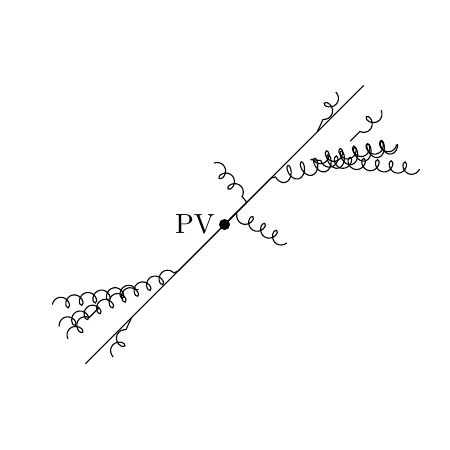
\begin{tikzpicture}
\def\Lenght{2.5}
\def\qangle{45}
\def\antiqangle{\qangle+180}

\clip (-\Lenght,-\Lenght) rectangle (\Lenght,\Lenght) ;

\fill (0,0) circle (2pt);
\draw (0,0) node [left] {PV} ;

\draw (0,0) --+ (\qangle:\Lenght) node [left] {\quark} ;
\draw (0,0) --+ (\antiqangle:\Lenght) node [right] {\antiquark} ;


\def\Lfrac{3}
\draw (0,0) --+ (\qangle:\Lenght/\Lfrac) coordinate (g1) ;
\draw (g1) + (\qangle-30:\Lenght-\Lenght/\Lfrac) coordinate (g2) ;
\draw [decoration={aspect=0.6, segment length=1.75mm, amplitude=1mm,coil},decorate] (g2) -- (g1) ;

\draw (g1) + (\qangle-20:{(\Lenght-\Lenght/\Lfrac)/(\Lfrac/2)}) coordinate (g3) ;
\draw (g3) + (\qangle:{\Lenght-\Lenght/\Lfrac-(\Lenght-\Lenght/\Lfrac)/(\Lfrac/2)}) coordinate (g4) ;
\draw [decoration={aspect=0.8, segment length=1.75mm, amplitude=.75mm,coil},decorate] (g4) -- (g3) ;

\draw (g1) + (\qangle-20:{(\Lenght-\Lenght/\Lfrac)/(\Lfrac)}) coordinate (g3) ;
\draw (g3) + (\qangle-35:{\Lenght-\Lenght/\Lfrac-(\Lenght-\Lenght/\Lfrac)/(\Lfrac)}) coordinate (g4) ;
\draw [decoration={aspect=0.8, segment length=1.75mm, amplitude=.75mm,coil},decorate] (g4) -- (g3) ;

\draw (g3) + (\qangle-50:{\Lenght-\Lenght/\Lfrac-(\Lenght-\Lenght/\Lfrac)/(\Lfrac*2)}) coordinate (g4) ;
\draw [decoration={aspect=0.8, segment length=1.75mm, amplitude=.75mm,coil},decorate] (g4) -- (g3) ;

\draw (g1) + (\qangle:{(\Lenght-\Lenght/\Lfrac)/(2*\Lfrac/3)}) coordinate (g3) ;
\draw (g3) + (\qangle+20:{\Lenght-\Lenght/\Lfrac-(\Lenght-\Lenght/\Lfrac)/(\Lfrac/2)}) coordinate (g4) ;
\draw [decoration={aspect=0.8, segment length=1.75mm, amplitude=.75mm,coil},decorate] (g4) -- (g3) ;

%% qbar shower
\draw (0,0) --+ (\antiqangle:\Lenght/\Lfrac) coordinate (g1) ;
\draw (g1) + (\antiqangle-20:\Lenght-\Lenght/\Lfrac) coordinate (g2) ;
\draw [decoration={aspect=0.8, segment length=1.75mm, amplitude=.75mm,coil},decorate] (g2) -- (g1) ;

\draw (g1) + (\antiqangle-20:{(\Lenght-\Lenght/\Lfrac)/(\Lfrac/2)}) coordinate (g3) ;
\draw (g3) + (\antiqangle:{\Lenght-\Lenght/\Lfrac-(\Lenght-\Lenght/\Lfrac)/(\Lfrac/2)}) coordinate (g4) ;
\draw [decoration={aspect=0.8, segment length=1.75mm, amplitude=.75mm,coil},decorate] (g4) -- (g3) ;

\draw (g1) + (\antiqangle-20:{(\Lenght-\Lenght/\Lfrac)/(\Lfrac)}) coordinate (g3) ;
\draw (g3) + (\antiqangle-35:{\Lenght-\Lenght/\Lfrac-(\Lenght-\Lenght/\Lfrac)/(\Lfrac)}) coordinate (g4) ;
\draw [decoration={aspect=0.8, segment length=1.75mm, amplitude=.75mm,coil},decorate] (g4) -- (g3) ;

%\draw (g3) + (\antiqangle-50:{\Lenght-\Lenght/\Lfrac-(\Lenght-\Lenght/\Lfrac)/(\Lfrac*2)}) coordinate (g4) ;
%\draw [decoration={aspect=0.8, segment length=1.75mm, amplitude=.75mm,coil},decorate] (g4) -- (g3) ;

\draw (g1) + (\antiqangle:{(\Lenght-\Lenght/\Lfrac)/(2*\Lfrac/3)}) coordinate (g3) ;
\draw (g3) + (\antiqangle+20:{\Lenght-\Lenght/\Lfrac-(\Lenght-\Lenght/\Lfrac)/(\Lfrac/2)}) coordinate (g4) ;
\draw [decoration={aspect=0.8, segment length=1.75mm, amplitude=.75mm,coil},decorate] (g4) -- (g3) ;

%% soft gluons
\draw (0,0) --+ (\qangle:.2) coordinate (g1) ;
\draw (g1) + (\qangle-75:.75) coordinate (g2) ;
\draw [decoration={aspect=0.8, segment length=1.75mm, amplitude=.75mm,coil},decorate] (g2) -- (g1) ;

\draw (0,0) --+ (\qangle:.4) coordinate (g1) ;
\draw (g1) + (\qangle+85:.65) coordinate (g2) ;
\draw [decoration={aspect=0.8, segment length=1.75mm, amplitude=.75mm,coil},decorate] (g2) -- (g1) ;

\end{tikzpicture}}

\caption[Formation de deux gerbes partoniques.]{Formation de deux gerbes partoniques à partir d'une paire de quarks formée au vertex primaire (PV).}
\label{fig-parton_shower}
\end{figure}

\subsubsection{Hadronisation}\label{chapter-MSSM-formation_jets-subsec-hadronisation}
Lorsque des partons en émettent d'autres, la conservation de l'énergie implique que chaque particule, individuellement, possède une énergie de plus en plus petite.
Or $\alpha_s$ augmente lorsque l'échelle d'énergie diminue et en-deçà de quelques centaines de \SI{}{\MeV}, $\alpha_s$ diverge.
Le phénomène de confinement de couleur réapparaît et la gerbe partonique subit le phénomène d'hadronisation.
Un flux collimé de hadrons, particules de charge de couleur nulle composées de partons, est alors obtenu.
Certains de ces hadrons peuvent comporter des quarks de deuxième ou troisième génération. Ils sont alors instables et peuvent être amenés à se désintégrer, auquel cas ce sont leurs produits de désintégration qui sont observés dans le détecteur.
\par Le phénomène d'hadronisation ayant lieu lorsque $\alpha_s\gg1$, il n'est pas possible de réaliser des calculs perturbatifs. Afin de décrire ce phénomène, il faut avoir recours à des modèles paramétriques. Deux d'entre eux sont décrits ci-après,
le modèle des cordes de Lund~\cite{Andersson_parton_fragmentation}
et
le modèle d'agglomération hadronique~\cite{Winter_2004}.
\paragraph{Modèle des cordes de Lund}\label{chapter-MSSM-formation_jets-subsec-hadronisation-subsubsec-Lund}
Dans le modèle des cordes de Lund~\cite{Andersson_parton_fragmentation}, les quarks sont reliés en paires $\quark\antiquark$ par des \og cordes \fg{} de couleur, de tension $\kappa \simeq \SI{1}{\GeV.\femto\meter^{-1}}$, comme sur la figure~\ref{subfig-Lund2}. Les gluons sont décrits comme des nœuds des cordes de couleur.
\begin{figure}[h]
\centering
\subcaptionbox{Les deux quarks issus de la collision se séparent à grande vitesse.\label{subfig-Lund1}}[.3\textwidth]
{\begin{tikzpicture}
\draw (-.15,0) node (q1) {} ;
\draw (+.15,0) node (q2) {} ;

\draw [black, fill=ltcolorred3] (q1) circle (3pt);
\draw [black, fill=ltcolorcyan3] (q2) circle (3pt);

\draw [very thick, -latex] (q1) --+ (-.75,0);
\draw [very thick, -latex] (q2) --+ (+.75,0);

\draw (q1) node [above] {\quark};
\draw (q2) node [above] {\antiquark};
\end{tikzpicture}}
\hfill
\subcaptionbox{Une \og corde \fg{} de flux de couleur se forme entre les deux quarks.\label{subfig-Lund2}}[.3\textwidth]
{\begin{tikzpicture}
\draw (-.95,0) node (q1) {} ;
\draw (+.95,0) node (q2) {} ;

\foreach \qa/\qb in {
q1/q2%
}{
\foreach \Dangle in {-15,0,15}{
\draw [thick, ltcolormagenta] (\qa) to  [in=180-\Dangle, out=\Dangle] (\qb);
}
}

\draw [black, fill=ltcolorred3] (q1) circle (3pt);
\draw [black, fill=ltcolorcyan3] (q2) circle (3pt);

\draw [very thick, -latex] (q1) --+ (-.75,0);
\draw [very thick, -latex] (q2) --+ (+.75,0);

\draw (q1) node [above] {\quark};
\draw (q2) node [above] {\antiquark};
\end{tikzpicture}}
\hfill
\subcaptionbox{L'énergie potentielle de la corde est suffisamment grande pour former de nouvelles paires de quarks.\label{subfig-Lund3}}[.3\textwidth]
{\begin{tikzpicture}
\draw (-1.05,0) node (q1) {} ;
\draw (+1.05,0) node (q2) {} ;


\draw (-.25,0) node (q3) {} ;
\draw (+.25,0) node (q4) {} ;

\foreach \qa/\qb in {
q1/q3,%
q4/q2%
}{
\foreach \Dangle in {-15,0,15}{
\draw [thick, ltcolormagenta] (\qa) to  [in=180-\Dangle, out=\Dangle] (\qb);
}
}

\draw [black, fill=ltcolorred3] (q1) circle (3pt);
\draw [black, fill=ltcolorcyan3] (q2) circle (3pt);
\draw [black, fill=ltcoloryellow3] (q3) circle (3pt);
\draw [black, fill=ltcolorblue3] (q4) circle (3pt);

\draw [very thick, -latex] (q1) --+ (-.75,0);
\draw [very thick, -latex] (q2) --+ (+.75,0);

\draw (q1) node [above] {\quark};
\draw (q2) node [above] {\antiquark};
\draw (q3) node [above] {$\antiquark'$};
\draw (q4) node [above] {$\quark'$};
\end{tikzpicture}}

\vspace{\baselineskip}

\subcaptionbox{Le processus se répète tant qu'il y a suffisamment d'énergie pour générer une paire de quarks.\label{subfig-Lund4}}[.45\textwidth]
{\begin{tikzpicture}
\draw (-1.95,0) node (q1) {} ;
\draw (+1.95,0) node (q2) {} ;

\draw (-.45,0) node (q3) {} ;
\draw (+.45,0) node (q4) {} ;

\draw (-1.05,0) node (q5) {} ;
\draw (+1.05,0) node (q6) {} ;

\draw (-1.35,0) node (q7) {} ;
\draw (+1.35,0) node (q8) {} ;

\foreach \qa/\qb in {
q1/q7,%
q5/q3,%
q4/q6,%
q8/q2%
}{
\foreach \Dangle in {-15,0,15}{
\draw [thick, ltcolormagenta] (\qa) to  [in=180-\Dangle, out=\Dangle] (\qb);
}
}

\draw [black, fill=ltcolorred3] (q1) circle (3pt);
\draw [black, fill=ltcolorcyan3] (q2) circle (3pt);
\draw [black, fill=ltcoloryellow3] (q3) circle (3pt);
\draw [black, fill=ltcolorblue3] (q4) circle (3pt);
\draw [black, fill=ltcolorgreen3] (q5) circle (3pt);
\draw [black, fill=ltcoloryellow3] (q6) circle (3pt);
\draw [black, fill=ltcolormagenta3] (q7) circle (3pt);
\draw [black, fill=ltcolorblue3] (q8) circle (3pt);

\draw [very thick, -latex] (q1) --+ (-.75,0);
\draw [very thick, -latex] (q2) --+ (+.75,0);

\draw (q1) node [above] {\quark};
\draw (q2) node [above] {\antiquark};
\draw (q3) node [above] {$\antiquark'$};
\draw (q4) node [above] {$\quark'$};
\draw (q5) node [above] {$\quark''$};
\draw (q6) node [above] {$\antiquark'''$};
\draw (q7) node [above] {$\antiquark''$};
\draw (q8) node [above] {\ $\quark'''$};
\end{tikzpicture}}
\hfill
\subcaptionbox{Des hadrons non colorés sont formés se forment à partir des quarks de basse énergie.\label{subfig-Lund5}}[.45\textwidth]
{\begin{tikzpicture}
\foreach \x/\y in {
1/0,1.1/-.05,%
1.9/.1,2/.15,%
1.4/.2,1.4/.4,1.55/.3,%
-1/0,-1.1/-.05,%
-1.85/.1,-2/.15,-1.95/.035,%
-1.4/.2,-1.25/.3,-1.4/.4%
}
{
\draw [black, fill=ltcolorgray2] (\x,\y-.125) circle (3pt);
}

\draw [very thick, -latex] (-2.25,0) --+ (-.75,0);
\draw [very thick, -latex] (-2.2,-.3) --+ (-.75,-.1);
\draw [very thick, -latex] (-2.25,.3) --+ (-.75,.1);

\draw [very thick, -latex] (2.25,0) --+ (+.75,0);
\draw [very thick, -latex] (2.25,-.3) --+ (+.75,-.1);
\draw [very thick, -latex] (2.25,.3) --+ (+.75,.1);
\end{tikzpicture}}

\caption[Formation de jets dans le cadre du modèle des cordes de Lund.]{Processus de formation de deux jets dans le cadre du modèle des cordes de Lund.}
\label{fig-Lund}
\end{figure}
\par Lorsque deux charges colorées s'éloignent, l'énergie potentielle augmente.
Une fois que l'énergie potentielle est suffisamment grande, une nouvelle paire $\quark'\antiquark'$ est créée (fig.~\ref{subfig-Lund3}), avec une probabilité proportionnelle à $\exp(-\frac{\pi}{\kappa} m_{\quark'})$; la probabilité d'obtenir des quarks lourds par ce processus est donc très faible.
Le partage de l'énergie entre les paires de quarks est régie par une fonction de partition dont les paramètres sont estimés expérimentalement.
\paragraph{Modèle d'agglomération hadronique}\label{chapter-MSSM-formation_jets-subsec-hadronisation-subsubsec-agglo_hadronique}
\begin{wrapfigure}{R}{8cm}
\centering
\begin{fmffile}{QCD_clustering_fragmentation}
\begin{fmfchar*}(50,60)
  \fmfleft{i1}
  \fmfrightn{o}{30}
  \fmf{boson,tension=10}{i1,v1}
  \fmf{phantom}{o3,v1,o27}
  \fmffreeze
  \fmf{phantom}{o3,v2}
  \fmf{plain}{v2,v4,v5,v1,v6,v7,v8}
  \fmf{phantom}{v8,o27}
  \fmffreeze
  \fmf{plain}{o1,v2}
  \fmf{plain}{v2,v3,v4,v5,v1,v6,v7,v8}
  \fmf{plain}{v8,o30}
  \fmffreeze
  \fmf{plain}{o3,v9,o4}
  \fmf{plain}{o5,v10,o6}
  \fmf{plain}{v9,v11,v10}
  \fmf{plain}{v11,v12}
  \fmf{plain}{v2,v16,v12,v13}
  \fmf{plain}{v13,v14,v15}
  \fmf{gluon}{v14,v4}
  \fmf{plain}{v15,v17,v17b,o9}
  \fmf{plain}{o10,v17b,o8}
  \fmf{plain,tension=4}{v17,v17c,v18}
  \fmf{plain}{v18,o11}
  \fmf{gluon}{v19,v5}
  \fmf{plain}{v20,v19,v18}
  \fmf{plain}{o16,v20}
  \fmf{plain,tension=4}{v20,v21,v22}
  \fmf{plain}{v22,o18}
  \fmf{plain}{v22,v23}
  \fmf{gluon, tension=2}{v6,v24}
  \fmf{gluon}{v24,v23}
  \fmf{gluon}{v25,v24}
  \fmf{plain}{v23,v26,v27,v28,v25}
  \fmf{plain}{v28,o20}
  \fmf{plain}{v26,v29,o21}
  \fmf{plain}{v29,o22}
  \fmf{plain}{v29,v30,o23}
  \fmf{plain}{v30,o24}
  \fmf{plain}{v25,v31}
  \fmf{plain,tension=4}{v31,v32,v8}
  \fmf{plain}{v31,v33}
  \fmf{plain}{o28,v33,o26}
  \fmfblob{.1w}{v16}
  \fmfblob{.1w}{v17c}
  \fmfblob{.1w}{v21}
  \fmfblob{.1w}{v27}
  \fmfblob{.1w}{v32}
  \fmfdot{v1,v4,v5,v6,v14,v19,v23,v24,v25}
  \fmflabel{ }{o1}
\end{fmfchar*}
\end{fmffile}
\caption[Formation de jets dans le cadre du modèle d'agglomération hadronique.]{Schématisation de l'hadronisation dans le cadre du modèle d'agglomération hadronique.}
\label{fig-agglo_hadronique}
\end{wrapfigure}
L'agglomération hadronique~\cite{Winter_2004} repose sur l'hypothèse de conservation des nombres quantiques ainsi que de l'énergie-impulsion entre les partons issus de la gerbe hadronique et les hadrons obtenus après hadronisation.
\par Dans un premier temps, les gluons de la gerbe partonique se désintègrent en paires $\quark\antiquark$. Les partons, uniquement des quarks à ce stade donc, se rassemblent dans un second temps en agglomérats de charge de couleur nulle, c'est le \og pré-confinement \fg.
Deux cas de figurent se présentent alors:
\begin{itemize}
\item la masse de l'agrégat est proche de celle d'un hadron, l'agrégat produit ce hadron;
\item la masse de l'agrégat n'est pas proche de celle d'un hadron et son énergie est supérieure à un seuil $Q_0$, cet agrégat se désintègre en agrégats plus petits et forme plusieurs hadrons.
\end{itemize}
Ce processus est illustré sur la figure~\ref{fig-agglo_hadronique}.

\subsubsection{Parton initial et caractéristiques du jet}
Selon le parton à l'origine du jet, ce dernier présente certaines caractéristiques, discutées ci-après.
Le parton n'est pas visible expérimentalement, mais les caractéristiques du jet obtenu permettent d'en estimer la saveur, comme exposé au chapitre~\refChLHCCMS.
\paragraph{Le quark~\quarkt} possède une durée de vie trop courte pour participer à l'hadronisation. Il se désintègre alors par interaction faible en un autre quark, très majoritairement un quark~\quarkb, et un boson \Wboson. Le nouveau quark issu de cette désintégration forme alors un jet.
\par Les autres quarks, \quarkd, \quarku, \quarks, \quarkc\ et~\quarkb, sont plus stables que le top et participent à l'hadronisation.
Ils se retrouvent donc confinés au sein des hadrons formés, éventuellement instables.
\paragraph{Le quark~\quarkb} ne forme pas de hadron stable et se désintègre en quark~\quarkc\ ou~\quarku\ par interaction faible.
Dans \SI{70}{\%} des cas, cette désintégration se fait avec émission d'une nouvelle paire de quarks $\quark\antiquark$ selon
\begin{equation}
\quarkb \to \quarkc\,\quark_d\antiquark_d
\msep
\antiquarkb \to \antiquarkc\,\quark_u\antiquark_u
\msep
\quarkb \to \quarku\,\quark_d\antiquark_d
\msep
\antiquarkb \to \antiquarku\,\quark_u\antiquark_u
\mend[,]
\end{equation}
où $q_d$ et $q_u$ désignent respectivement des quarks d'isospin faible bas et haut.
Le nombre de constituants du jet, ainsi que le nombre de traces déplacées, est alors plus important.
Dans \SI{30}{\%} des cas, la désintégration du quark $b$ se fait avec émission d'une paire de leptons, un électriquement chargé et le neutrino associé, \ie
\begin{equation}
\quarkb \to \quarkc\,\lepton^-\antineutrino_\ell
\msep
\antiquarkb \to \antiquarkc\,\lepton^+\neutrino_\ell
\msep
\quarkb \to \quarku\,\lepton^-\antineutrino_\ell
\msep
\antiquarkb \to \antiquarku\,\lepton^+\neutrino_\ell
\mend
\end{equation}
Le lepton chargé donne une signature caractéristique lors des collisions proton-proton du LHC.
\par Ces désintégrations font intervenir les modules des coefficients $V_{\quarkc\quarkb}$ ou $V_{\quarku\quarkb}$ de la matrice CKM, introduite dans la section~\ref{chapter-MS-MSSM-section-formalisme-subsec-EW-quarks}, dont les valeurs sont faibles; elles sont donc fortement supprimées.
Les hadrons contenant un quark~\quarkb\ ont ainsi une durée de vie $\tau$ de l'ordre de la picoseconde~\cite{B0s_lifetime,lifetimes_c_b_hadrons} et peuvent voyager sur une distance de l'ordre du millimètre.
Les traces des particules chargées issues de cette nouvelle désintégration proviennent donc d'un vertex secondaire (SV), différent du vertex primaire (PV).
Ces traces sont \og déplacées \fg.
Pour chacune d'entre elles, il est possible de déterminer le paramètre d'impact (IP) au vertex primaire, dont la valeur est typiquement plus grande que pour des traces provenant du vertex primaire, comme cela est illustré sur la figure~\ref{fig-chapter-CMS-section-jets_reco-subsec-flavor-SV_scheme}.
\begin{figure}[h]
\centering
\begin{tikzpicture}[scale=1.5]
\def\Bjetangle{30}
\def\Bhaddronangle{5}
\def\Bhaddronflight{.75}

\clip (-145:\Solenrin) rectangle (\Bjetangle:1.8*\Solenrin);

\foreach\jetangle in {120,-145}{
\printbigjetnolabel{9}{\jetangle}
\draw (\jetangle:2.75) node {jet} ;
}

\def\CurrentVertex{(\Bhaddronangle:\Bhaddronflight)}

\draw [thick, dotted] (0,0) -- \CurrentVertex ;

{
\def\jetcolor{ltcolorred}
\printjetnolabel{9}{\Bjetangle}
\draw [\jetcolor] (\Bjetangle:2)+(1.5,.75) node {traces déplacées};
}
\begin{scope}
\clip circle (\Solenrin);
\printantimuonnolabel{7}{\Bjetangle}
\end{scope}

\draw [\muoncolor] (\Bjetangle:4) +(0,{-2*\baselineskip}) node {lepton chargé};

\draw (\Bjetangle:4) + (-.125,-.5) circle (1.125);
\draw [-latex] (\Bjetangle:4) + (-.125,-1.625) --+ (-.125,-2) node [below] {jet de saveur lourde};

\draw (0,0) node [left] {PV} ;
\draw \CurrentVertex node [below right] {SV} ;

\fill (0,0) circle (2pt);
\fill \CurrentVertex circle (2pt);

\draw [dashed] \CurrentVertex --+ (\Bjetangle:-.8);

\draw [red, latex-latex] (0,0)--+ (-90+\Bjetangle:{\Bhaddronflight*sin(\Bjetangle-\Bhaddronangle)}) node [below right] {IP};
\end{tikzpicture}
\caption[Trois jets, dont un de saveur lourde.]{Trois jets, dont un de saveur lourde. Les particules composant ce jet proviennent d'un vertex secondaire (SV), différent du vertex primaire (PV) où a lieu la collision entre les protons et la formation du hadron lourd à l'origine du SV. Le paramètre d'impact (IP) est également indiqué. Réalisé à l'aide de CMSTransverseTikZ~\cite{CMSTransverseTikZ}.}
\label{fig-chapter-CMS-section-jets_reco-subsec-flavor-SV_scheme}
\end{figure}
\paragraph{Le quark~\quarkc} suit le même schéma que le quark~\quarkb. Cependant, la désintégration du quark~\quarkc\ en quark~\quarks\ selon
\begin{equation}
\quarkc \to \quarks\,\quark_u\antiquark_u
\msep
\antiquarkc \to \antiquarks\,\quark_d\antiquark_d
\msep
\quarkc \to \quarks\,\lepton^+\neutrino_\ell
\msep
\antiquarkc \to \antiquarks\,\lepton^-\antineutrino_\ell
\mend[,]
\end{equation}
fait intervenir le module du coefficient $V_{\quarkc\quarks}$ de la matrice CKM, proche de 1.
Les hadrons contenant un quark~\quarkc\ ont ainsi une durée de vie $\tau$ de inférieure à la picoseconde~\cite{lifetimes_c_b_hadrons} et il est plus difficile d'identifier les jets issus de quarks~\quarkc\ que ceux issus de quarks~\quarkb.
\paragraph{Les quarks~\quarkd, \quarku\ et~\quarks} forment des hadrons étant:
\begin{itemize}
\item très instables, par exemple les \pionnull, dont seuls les produits de désintégration sont observés;
\item faiblement instables, par exemple les \Kaonplus\ et les \Kaonnull, qui se propagent généralement jusque dans les parties sensibles du détecteur et peuvent donc être directement observés;
\item stables, par exemple les protons, qui sont directement observés dans le détecteur.
\end{itemize}
Dans tous les cas, les traces des particules chargées observées proviennent du PV, lieu de formation du quark initial.
Le phénomène décrit précédemment pour les quarks~\quarkb\ et~\quarkc\ n'est donc pas observable.
Les jets issus de ces trois types de quarks, les plus légers, sont ainsi regroupés sous la dénomination de \og jets légers \fg.
\paragraph{Les gluons} portent une charge de couleur plus importante que les quarks.
Les quarks portent en effet une couleur, les antiquarks une anticouleur et les gluons portent une couleur et une anticouleur.
Les jets initiés par des gluons comportement typiquement plus de particules électriquement chargées et sont moins collimés que les jets légers~\cite{CMS-PAS-JME-13-002}.
